\documentclass[../main]{subfiles}

\graphicspath{{../figures/}}

\begin{document}


% 図表の例:コーンペネトロメータを\reffig{fig:cone_penetrometer}に示す.
% \reftab{tab:traffic_cone_index}が示すように,各建設機械の走行に必要とされているコーン指数は既にわかっている.

\section{背景}
\label{sec:intro_background}
\subsection{石油精製プラント点検の現状}
\label{sec:intro_plant_current}
近年,地球温暖化の進行を抑えることを目的としたカーボンニュートラルの実現が求められているが,\reffig{oil_consumption}に示すように,石油を代表とする化石燃料は今後もエネルギー源として重要な役割を果たすことが予想される.\cite{ritchie2023energy}
原油の精製は,ガソリンやディーゼル燃料,ジェット燃料といった輸送エネルギー資源のほか,プラスチック,化学肥料,医薬品,合成繊維など様々な化学製品の製造に欠かせない工程であり,
\reffig{fig:view_plant}に示すような石油精製プラントはその中心的な役割を担っている.\cite{eneos2024}
このようなプラントには,多種多様なプロセスが含まれており,それを支えるポンプ\cite{Shvindin2008A}や熱交換器\cite{Abbasov2023PRIMARY},蒸留装置,反応器など,複雑かつ多岐にわたる設備が混在しており,
これらの装置が適切に機能することで,高品質なプロダクトの安定供給を可能としている.


また,保守作業はすべての産業において重要な要素であり,石油精製プラントにおいても例外ではない.
設備の老化から環境条件による劣化など,様々な要因により設備の故障が発生することがあり,これらのいかなる故障も,プロセスの停止による製造の遅れ,高額な修理費,さらには事故の発生といった深刻な問題を引き起こす可能性がある.
また,石油精製プラント内で扱われる化学物質は,可燃性のものが多く,事故の発生による火災や爆発のリスクが常に付きまとう.\cite{Tang2021}
そのため,設備の異常を早期に検知し,適切な対処を行うことが求められている.

現在,点検作業は人手によって行われ,通常,各石油化工施設には専属の現場作業員のグループが配置されており,昼夜を問わず1日に何度も巡回を行う.
こうした巡回中に現場作業員は施設全体を歩きながら,機械の包括的な点検を実施する.
表に示すように,点検の内容は圧力計の値を目視で確認したり,配管の腐食を探したり,ポンプやバルブなどの回転機械が発する異常な音を聞き分けることなど多岐にわたる.

しかし,これらの点検は人手によって行われており,プラント内では多くの設備が稼働しており,それらの設備が発する音量は非常に大きく,
このような環境下で異常音を聞き分けることは困難なタスクであり,作業員の熟練度に依存して,異常音を見逃す可能性がある.
更に,以上の理由を踏まえて現場作業員は多くの熟練点検員によって構成されているが,結果として,高額な人件費がかかることになる点,また
高齢化により,熟練点検員の数自体が減少している点などが人手による点検の課題として挙げられる.
これらの理由から,石油精製プラント内の音響点検を自動化することが求められている.

プラント内音響点検の自動化に向けて,Shukutaniらによって石油精製プラントを想定した移動ロボットの開発が行われている.
この移動ロボットは,クローラを用いて移動し,平地や階段を問わず移動できるように設計されている.
また,移動ロボットには異常の種類に応じて異なるセンサを搭載し,これらのセンサには,全天球可視カメラ,熱画像カメラ,可視監視カメラやマイクロフォンなどが含まれる.
更に,点検対称の区域内に存在する,可燃性ガスや液体の着火源になることを防ぐため,これらすべてのセンサには防爆仕様が適用されている.
\begin{table}[t]
  \caption{プラント内の異常の種類(株式会社ENEOSより提供)}
  \label{tab:plant_anomalies}
  \centering
  \begin{tabular}{lll}
    \toprule
    対象機器 & 監視対象 & 検査手法 \\
    \midrule
    \textbf{ポンプの異常} & ベアリング異音 & 聴覚 \\
                 & 漏洩による白煙発生 & 視覚、嗅覚 \\
                 & 漏洩による着火 & 視覚、嗅覚 \\
                 & オイラーのオイルレベル低下 & 視覚 \\
                 & 閉塞等による冷却水低下、喪失 & 触覚 \\
                 & 発熱 & 触覚 \\
    \midrule
    \textbf{配管異常} & 外面腐食の進行 & 視覚 \\
               & 保温板金の劣化 & 視覚 \\
               & 保温劣化による表面温度上昇 & 触覚 \\
               & 腐食によるガス・油漏洩 & 視覚、嗅覚 \\
               & フランジ部からのガス・油漏洩 & 視覚、嗅覚 \\
    \midrule
    \textbf{その他機器の異常} & 加熱炉の耐火煉瓦脱落による炉壁発熱 & 視覚 \\
                   & バルブの誤開閉 & 視覚 \\
    \midrule
    メータ読み込み & 圧力計、温度計等 & 視覚 \\
    \bottomrule
  \end{tabular}
\end{table}

\begin{figure}[t]
  \centering
  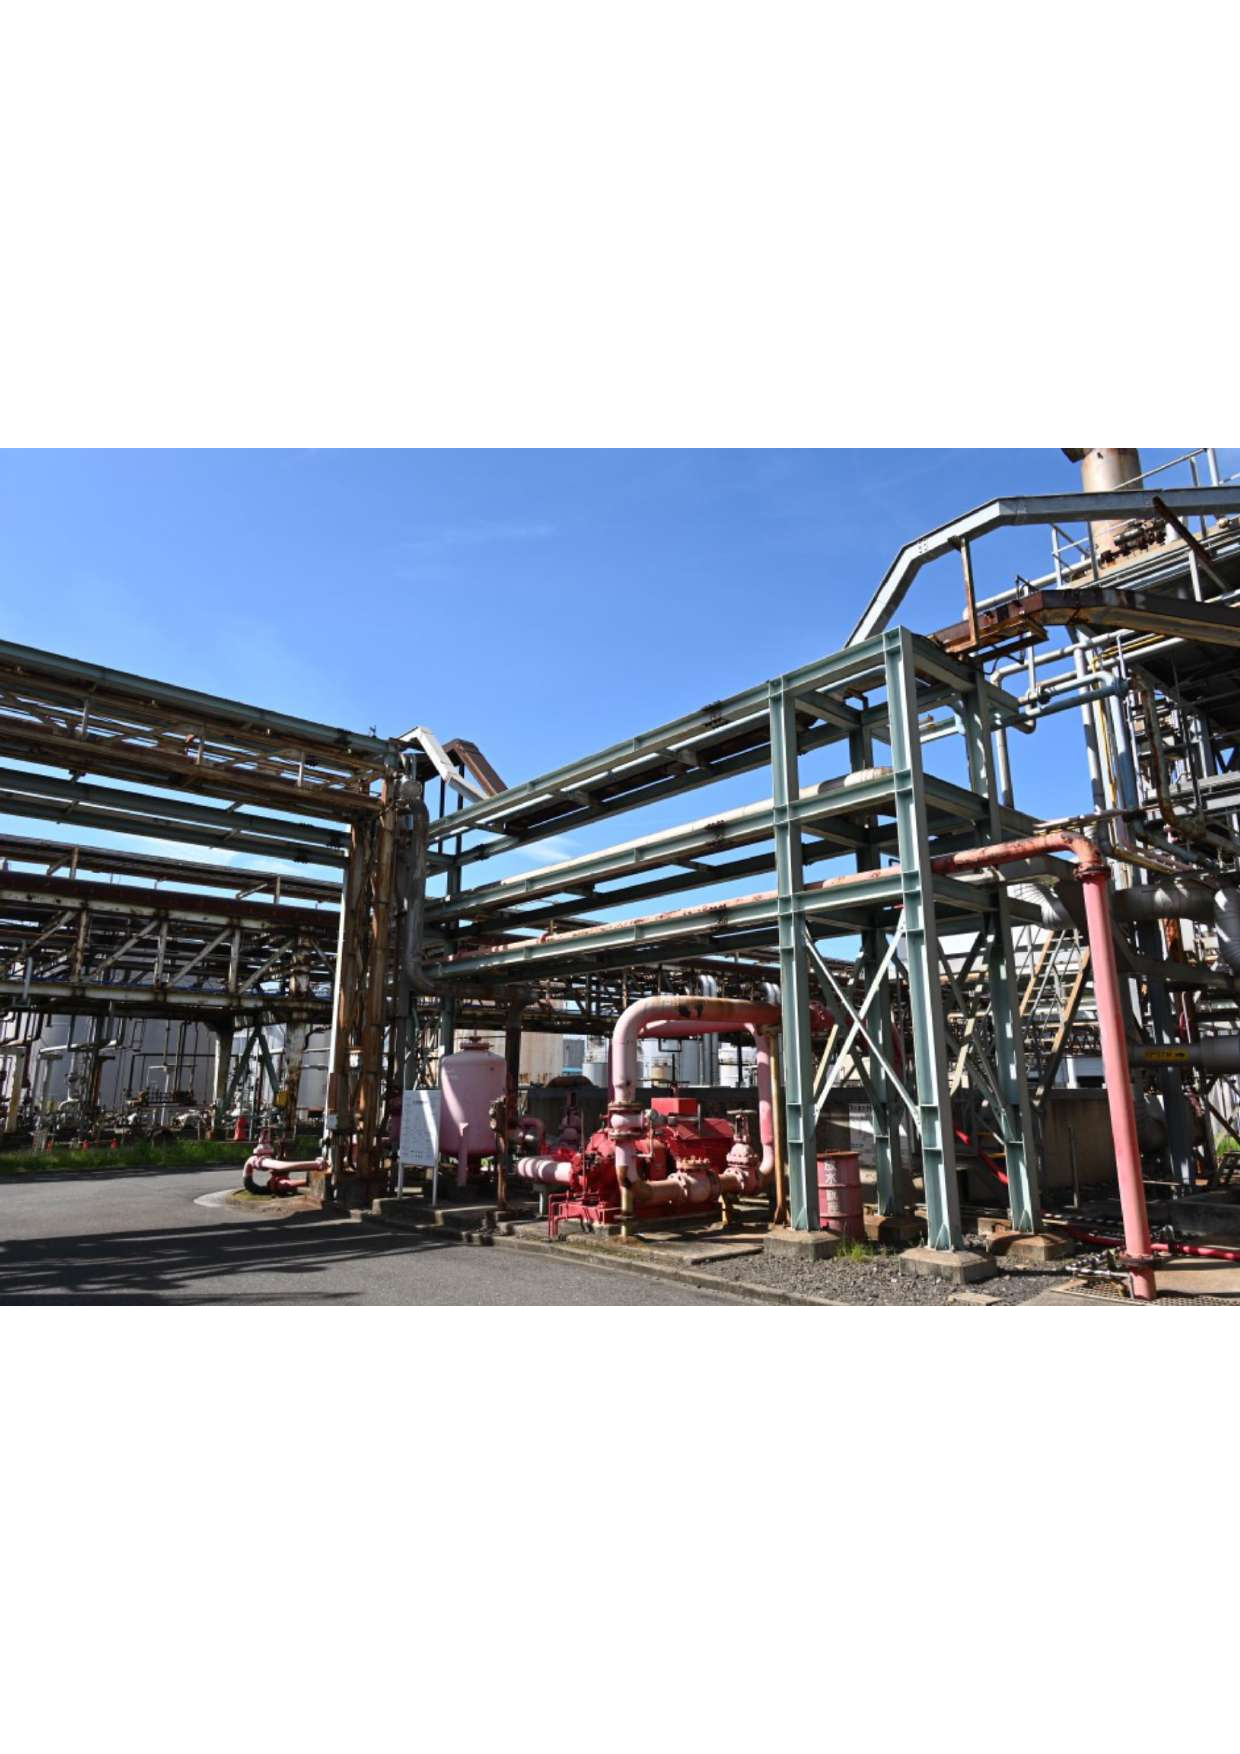
\includegraphics[keepaspectratio, width=0.5\linewidth]{chap1/view_plant.pdf}
  \caption{石油精製プラントの}
  \label{fig:view_plant}
\end{figure}
\subsection{プラント内音響点検の特徴}
\label{sec:intro_plant_characteristics}


前節で述べたように,人手によるプラント内の音響点検には,点検の質が作業員の熟練度に依存すること,高額な人件費がかかること,高齢化による熟練点検員の減少など複数の課題が存在し,
これらの課題を解決するためには,音響点検の自動化が求められている.
しかしながら,プラント内には,音響点検を困難にする様々な要因が存在し,本節ではその要因の説明のため,まずプラント内音響点検の特徴を述べ,それらの特徴に基づく課題を示す.

プラント内音響点検における対象は主に図1.4に示すように,ポンプやコンプレッサなど回転機器のベアリングの傷を検出することがあげられる.
また,これらのポンプなどの機器は図に示すように,数メールの区画に密集して,設置されており,それぞれの機器から発せられる音量は非常に大きく,
観測対象となる音は,これらの音が重なりあった音である.

これらの特徴から生じる課題として以下の2つがあげられる.
一つには,回転機器のベアリングの傷によって生じる異常音は,ベアリングの傷の深さや種類に依存して異なる性質を持ち,異なる異常音のデータが十分に取得することができないことがあげられる.
更に,異常音を発している機器を長時間観測することは,プラントの運転に支障をきたすことがあるため,不可能である.
加えて,異常の発生に関しても頻繁に発生するわけではなく,これらの多岐にわたる異常音を十分に取得することは困難であることがあげられる.

もう一つの課題として,図 に観測できるようにプラント内音響点検の対象となる箇所は,非常に狭い区間に多数の音を発する機器が密集しているため,
観測した異常音がどの機器によるものなのかということが明確になりにくいことがあげられる.
そのため,プラント内の音響点検では異常の有無の判別だけでなく,異常音の発生源を特定することが非常に重要である.
\end{document}
